\section{PottsModelInitP Struct Reference}
\label{structPottsModelInitP}\index{PottsModelInitP@{PottsModelInitP}}
{\tt \#include $<$PottsModel.h$>$}

Inheritance diagram for PottsModelInitP::\begin{figure}[H]
\begin{center}
\leavevmode
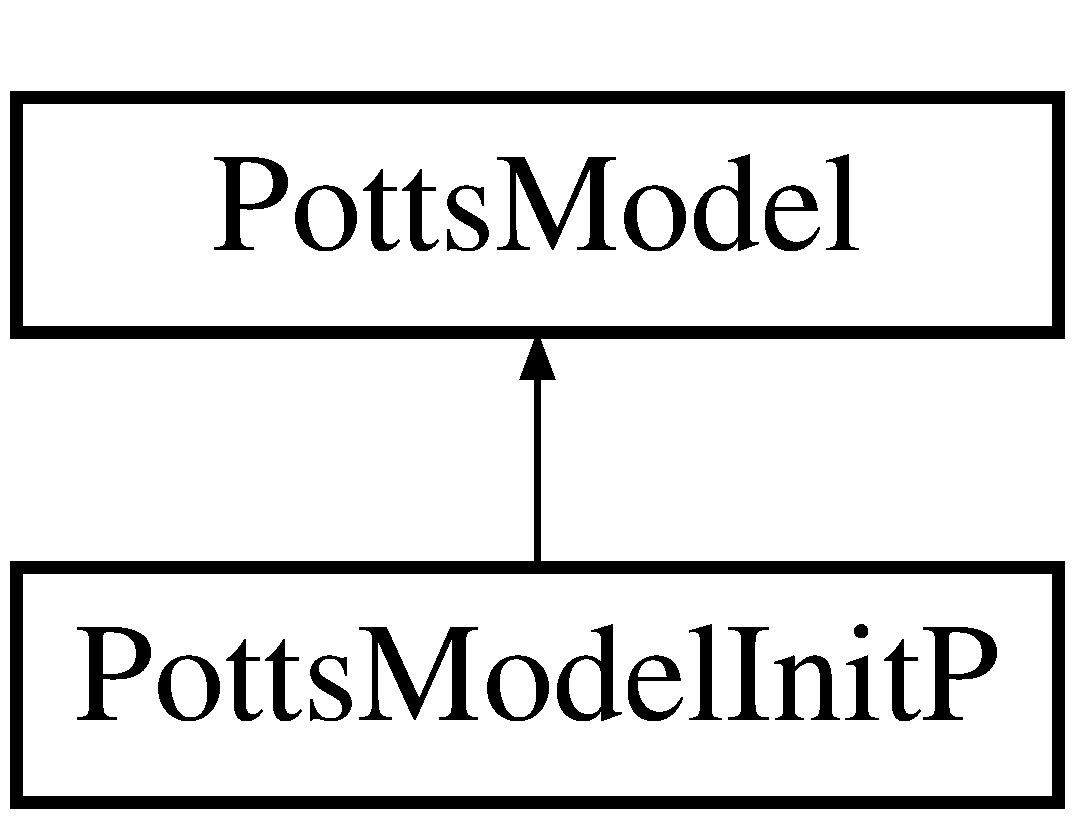
\includegraphics[height=2cm]{structPottsModelInitP}
\end{center}
\end{figure}
\subsection*{Public Member Functions}
\begin{CompactItemize}
\item 
{\bf PottsModelInitP} (int \_\-N1, int \_\-N2, int \_\-Q=2, {\bf LD} \_\-jSigma=0.1, {\bf LD} \_\-hSigma=0.1, int \_\-seed=0)
\item 
void {\bf setInitPseed} (int \_\-s)
\end{CompactItemize}
\subsection*{Public Attributes}
\begin{CompactItemize}
\item 
int {\bf init\_\-p\_\-seed}
\item 
gsl\_\-rng $\ast$ {\bf pRNG}
\end{CompactItemize}


\subsection{Detailed Description}
This class additionally provides the model init b(x\_\-0) which is assumed as factored into singletons - (note) 



\subsection{Constructor \& Destructor Documentation}
\index{PottsModelInitP@{PottsModelInitP}!PottsModelInitP@{PottsModelInitP}}
\index{PottsModelInitP@{PottsModelInitP}!PottsModelInitP@{PottsModelInitP}}
\subsubsection{\setlength{\rightskip}{0pt plus 5cm}PottsModelInitP::PottsModelInitP (int {\em \_\-N1}, int {\em \_\-N2}, int {\em \_\-Q} = {\tt 2}, {\bf LD} {\em \_\-jSigma} = {\tt 0.1}, {\bf LD} {\em \_\-hSigma} = {\tt 0.1}, int {\em \_\-seed} = {\tt 0})\hspace{0.3cm}{\tt  [inline]}}\label{structPottsModelInitP_da6e72d249ce377e013b20535df3461b}




\subsection{Member Function Documentation}
\index{PottsModelInitP@{PottsModelInitP}!setInitPseed@{setInitPseed}}
\index{setInitPseed@{setInitPseed}!PottsModelInitP@{PottsModelInitP}}
\subsubsection{\setlength{\rightskip}{0pt plus 5cm}void PottsModelInitP::setInitPseed (int {\em \_\-s})\hspace{0.3cm}{\tt  [inline]}}\label{structPottsModelInitP_f149dcc6fad10c198c9c41cad879b947}




\subsection{Member Data Documentation}
\index{PottsModelInitP@{PottsModelInitP}!init_p_seed@{init\_\-p\_\-seed}}
\index{init_p_seed@{init\_\-p\_\-seed}!PottsModelInitP@{PottsModelInitP}}
\subsubsection{\setlength{\rightskip}{0pt plus 5cm}int {\bf PottsModelInitP::init\_\-p\_\-seed}}\label{structPottsModelInitP_79d6d88d4ebd7a41e14c98f264049c2e}


\index{PottsModelInitP@{PottsModelInitP}!pRNG@{pRNG}}
\index{pRNG@{pRNG}!PottsModelInitP@{PottsModelInitP}}
\subsubsection{\setlength{\rightskip}{0pt plus 5cm}gsl\_\-rng$\ast$ {\bf PottsModelInitP::pRNG}}\label{structPottsModelInitP_3a7ad4aa95ce6f7fc96b73399aa9b011}




The documentation for this struct was generated from the following file:\begin{CompactItemize}
\item 
inc/{\bf PottsModel.h}\end{CompactItemize}
